\section{Atividades}

\subsection{Atividade 1 -- Levantamento de Informações}

\paragraph{}
O primeiro passo consistiu em acessar a máquina alvo utilizando o serviço SSH e
as credenciais obtidas em atividades anteriores.

\paragraph{}
Após o acesso inicial, foram utilizadas as ferramentas \texttt{LinEnum} e
\texttt{LinPEAS} para automatizar o processo de enumeração do sistema,
permitindo identificar configurações inseguras, permissões inadequadas e
possíveis vetores de escalação de privilégios.

\paragraph{}
As ferramentas foram transferidas da máquina atacante para a máquina alvo por
meio de um servidor HTTP temporário e através do protocolo \texttt{SCP},
demonstrando diferentes técnicas de transferência de arquivos em ambientes de
pentest.

\paragraph{}
Após a execução dos scripts, foram gerados relatórios contendo informações sobre
usuários, grupos, permissões de arquivos, configurações do \texttt{sudo},
presença de containers Docker e tarefas agendadas no sistema.

\paragraph{}
A análise dos relatórios revelou diversos pontos potencialmente exploráveis,
incluindo permissões incorretas nos arquivos \texttt{/etc/passwd} e
\texttt{/etc/shadow}, permissões de execução via \texttt{sudo} e associação do
usuário ao grupo \texttt{docker}.

\subsection{Atividade 2 -- Escalação de Privilégios por Arquivos Críticos}

\paragraph{}
Nesta etapa foram exploradas configurações incorretas relacionadas aos arquivos
críticos \texttt{/etc/passwd} e \texttt{/etc/shadow}, responsáveis pelo controle
de usuários e autenticação do sistema operacional.

\paragraph{}
A análise das permissões demonstrou que qualquer usuário possuía permissão de
escrita no arquivo \texttt{/etc/passwd} e permissão de leitura no arquivo
\texttt{/etc/shadow}, situação que representa uma grave falha de segurança.

\paragraph{}
Inicialmente foi realizada a criação de um novo usuário privilegiado através da
inserção manual de uma entrada no arquivo \texttt{/etc/passwd}, utilizando uma
senha previamente convertida para o formato de hash compatível com o sistema.

\paragraph{}
Após a criação da nova conta, foi possível autenticar-se utilizando a senha
definida e obter acesso com privilégios equivalentes ao usuário
\texttt{root}.

\paragraph{}
Em seguida foi explorada a possibilidade de leitura do arquivo
\texttt{/etc/shadow}, permitindo a extração das hashes de senhas armazenadas no
sistema.

\paragraph{}
As hashes obtidas foram submetidas a ataques de quebra utilizando a ferramenta
\texttt{John the Ripper}, possibilitando a recuperação de credenciais válidas e
o acesso a contas adicionais do sistema.

\begin{figure}[H]
  \centering
  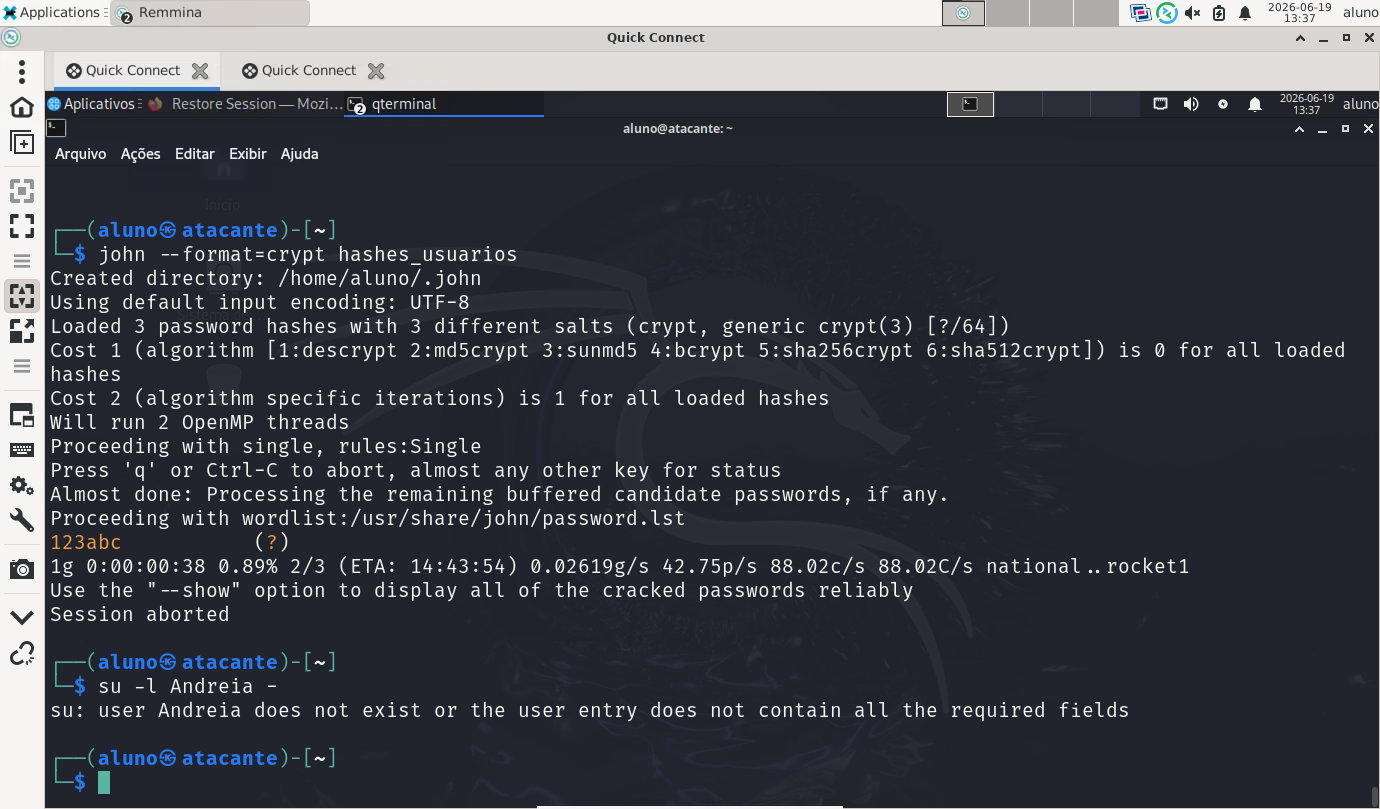
\includegraphics[width=0.95\textwidth]{./fig/passwd-shadow-privesc.png}
  \caption{Escalação de privilégios explorando permissões incorretas nos
  arquivos \texttt{/etc/passwd} e \texttt{/etc/shadow} usando \texttt{john}
  para revelar a senha de \textit{Andreia}.}
\end{figure}

\subsection{Atividade 3 -- Escalação de Privilégios Utilizando Sudo}

\paragraph{}
Após a obtenção das credenciais da usuária \texttt{Andreia}, foi realizada uma
análise das permissões configuradas no mecanismo \texttt{sudo}.

\paragraph{}
A consulta das permissões disponíveis revelou que a usuária possuía autorização
para executar o editor \texttt{vim} com privilégios elevados.

\paragraph{}
Embora o comando autorizado aparentasse ser limitado, foi verificado que o
\texttt{vim} permite a execução de comandos arbitrários do sistema operacional,
possibilitando a obtenção de uma shell privilegiada.

\paragraph{}
Por meio dos recursos internos do editor foi possível executar comandos como
usuário \texttt{root}, resultando na obtenção de acesso administrativo ao
sistema.

\paragraph{}
A atividade demonstrou que a autorização de programas aparentemente inofensivos
via \texttt{sudo} pode introduzir riscos significativos quando suas
funcionalidades não são devidamente avaliadas.

\begin{figure}[H]
  \centering
  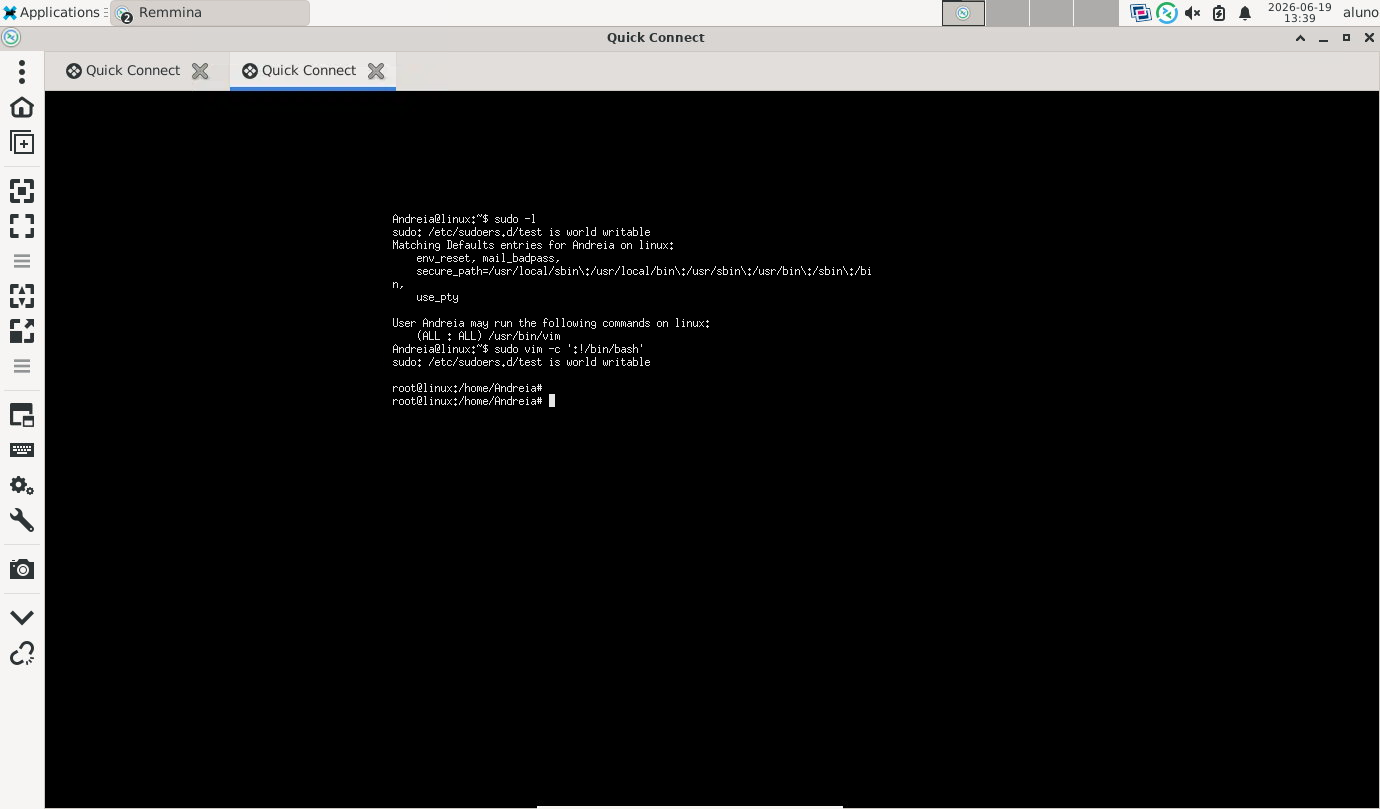
\includegraphics[width=0.95\textwidth]{./fig/sudo-vim-privesc.png}
  \caption{Obtenção de shell privilegiada explorando permissões de execução
  do editor \texttt{vim} através do \texttt{sudo}.}
\end{figure}

\subsection{Atividade 4 -- Escalação de Privilégios Utilizando Docker}

\paragraph{}
A última técnica explorada baseou-se na associação da usuária ao grupo
\texttt{docker}, condição identificada durante a fase de enumeração.

\paragraph{}
Foi verificado que o usuário possuía permissão para executar containers
arbitrários utilizando o mecanismo Docker instalado no sistema.

\paragraph{}
Inicialmente foram realizados testes de execução de containers para validar as
permissões disponíveis e compreender o nível de acesso obtido dentro do
ambiente isolado.

\paragraph{}
Posteriormente foi criado um container com o diretório raiz do sistema hospedeiro
montado em seu sistema de arquivos interno, permitindo acesso direto aos
arquivos do host.

\paragraph{}
A partir desse acesso foi possível criar um binário com permissões SUID
associadas ao usuário \texttt{root}, possibilitando a execução de comandos com
privilégios elevados fora do ambiente do container.

\paragraph{}
O procedimento resultou na obtenção de acesso administrativo ao sistema
hospedeiro, demonstrando como a associação indevida ao grupo \texttt{docker}
equivale, na prática, à concessão de privilégios de administrador.

\begin{figure}[H]
  \centering
  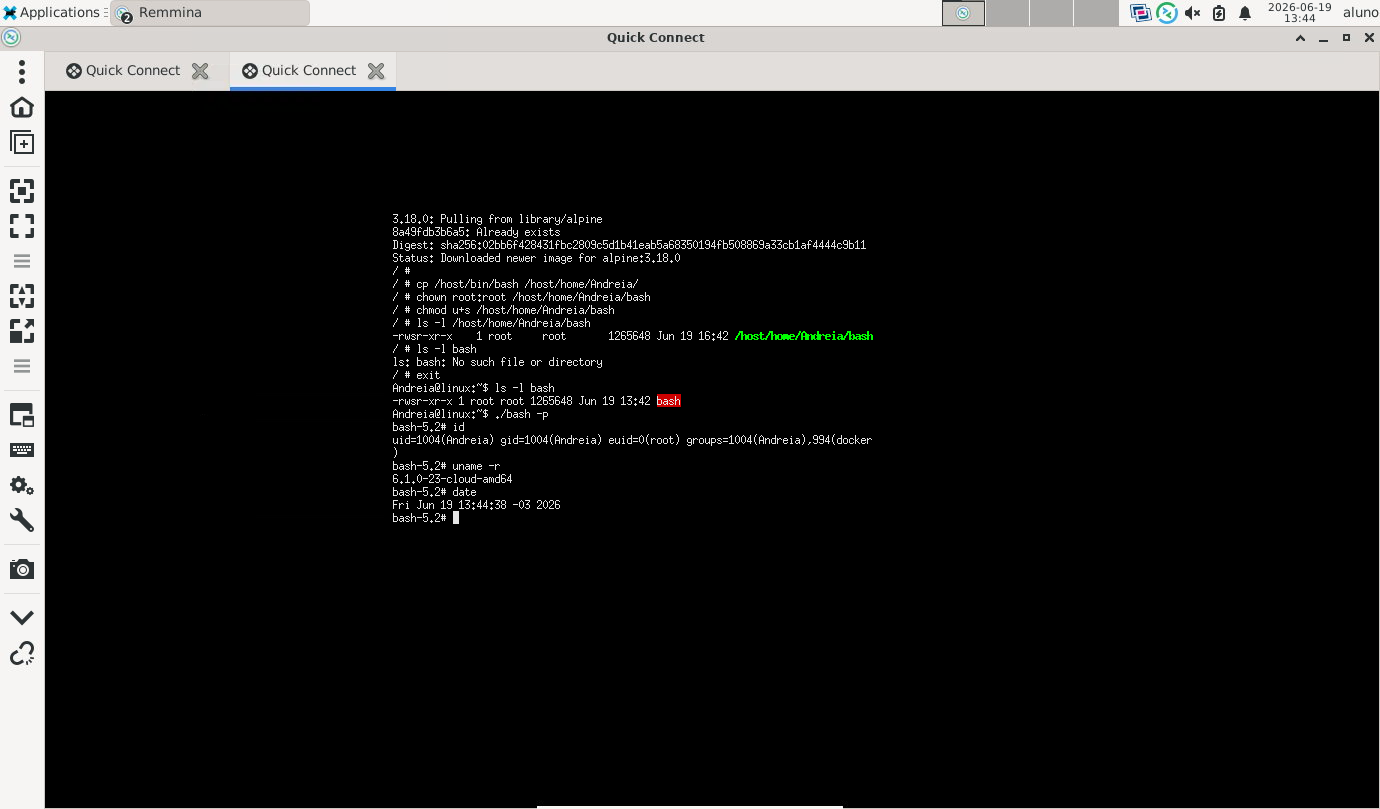
\includegraphics[width=0.95\textwidth]{./fig/docker-privesc.png}
  \caption{Escalação de privilégios explorando permissões de execução de
  containers Docker.}
\end{figure}

\subsection{Atividade 5 -- Escalação de Privilégios Abusando de Cron Mal Configurado}

\paragraph{}
Nesta atividade foi explorada uma vulnerabilidade relacionada à configuração
insegura de tarefas agendadas pelo serviço \texttt{cron}.

\paragraph{}
Inicialmente foram analisados os relatórios gerados pelas ferramentas
\texttt{LinEnum} e \texttt{PEASS}, que permitiram identificar a existência de
tarefas agendadas executadas com privilégios elevados e localizar arquivos de
configuração relacionados ao mecanismo de agendamento do sistema.

\paragraph{}
Embora as ferramentas tenham apresentado informações sobre os diretórios e
arquivos utilizados pelo \texttt{cron}, foi necessária uma análise manual das
configurações para identificar potenciais oportunidades de exploração.

\paragraph{}
Durante a inspeção dos arquivos presentes em \texttt{/etc/cron.d}, foi
identificada uma rotina de backup executada periodicamente pelo usuário
\texttt{root}, utilizando um script personalizado localizado em
\texttt{/usr/local/bin/backup.sh}.

\paragraph{}
A análise das permissões do arquivo revelou que qualquer usuário possuía
permissão de escrita sobre o script, permitindo sua modificação mesmo sem
privilégios administrativos.

\paragraph{}
Aproveitando essa configuração inadequada, foram inseridos comandos adicionais
no script de backup com o objetivo de criar uma cópia do interpretador
\texttt{bash}, atribuindo sua propriedade ao usuário \texttt{root} e
habilitando o bit SUID.

\paragraph{}
Como a tarefa era executada automaticamente pelo \texttt{cron} com privilégios
elevados, os comandos inseridos foram processados pelo sistema durante a
próxima execução agendada.

\paragraph{}
Após a execução da tarefa, foi verificado que o binário criado possuía
propriedade do usuário \texttt{root} e estava configurado com permissões SUID,
permitindo sua utilização para obtenção de privilégios elevados.

\paragraph{}
Por fim, o binário foi executado utilizando a opção apropriada para preservar
os privilégios efetivos, resultando na obtenção de uma shell com permissões de
\texttt{root}.

\paragraph{}
A atividade demonstrou como tarefas automatizadas executadas por usuários
privilegiados podem representar um vetor crítico de escalonamento de
privilégios quando scripts ou arquivos associados possuem permissões de escrita
inadequadas.
